\documentclass[10pt]{beamer}
\setbeamerfont{headline}{size=\footnotesize}

\mode<presentation>{
\usetheme{Montpellier}
\setbeamercovered{transparent}
\usecolortheme{lsc}
}

\mode<handout>{
  \usepackage[bar]{beamerthemetree}
  \beamertemplatesolidbackgroundcolor{black!5}
}

\usepackage[english,brazil]{babel}
\usepackage[utf8]{inputenc}
\usepackage[T1]{fontenc}
\usepackage{amsmath, amssymb}
\usepackage{graphicx}
\usepackage{booktabs}
\usepackage{array}
\usepackage{tabularx}
\usepackage{xcolor}
\usepackage{colortbl}
\usepackage{caption}
\usepackage{transparent}
\usepackage{pdfpages}
\usepackage{url}
\usepackage{fontawesome5}
\usepackage{ccicons}
\usepackage{listings}
\usepackage{tikz}
\usepackage{pgfplots}
\usetikzlibrary{shapes.geometric, arrows.meta, positioning, calc, fit, backgrounds, matrix, decorations.pathreplacing}
\usetikzlibrary{pgfplots.groupplots}
\pgfplotsset{compat=1.16, every axis/.append style={tick label style={font=\tiny}, label style={font=\scriptsize}, legend style={font=\tiny}}}

\captionsetup{font=footnotesize, labelfont=bf}

% Cores
\definecolor{azul}{RGB}{0,76,128}
\definecolor{laranja}{RGB}{225,115,20}
\definecolor{verde}{RGB}{40,140,70}
\definecolor{vermelho}{RGB}{190,40,40}
\definecolor{codegreen}{rgb}{0,0.6,0}
\definecolor{codegray}{rgb}{0.5,0.5,0.5}
\definecolor{codepurple}{rgb}{0.58,0,0.82}
\definecolor{backcolour}{rgb}{0.95,0.95,0.92}

\lstdefinestyle{mystyle}{
    frame=single, framesep=4pt, xleftmargin=0pt, xrightmargin=0pt,
    backgroundcolor=\color{backcolour},
    commentstyle=\color{codegreen}, keywordstyle=\color{magenta},
    stringstyle=\color{codepurple}, basicstyle=\scriptsize\ttfamily,
    breaklines=true, keepspaces=true, showstringspaces=false, tabsize=2,
    upquote=true, language=Python
}
\lstset{style=mystyle}

% Estilos TikZ reutilizáveis
\tikzset{
  caixa/.style={draw=azul, rounded corners=2pt, fill=azul!10, align=center, font=\footnotesize, inner sep=3pt, minimum height=6mm},
  seta/.style={-{Stealth[length=2.2mm]}, thick, azul!70!black},
  neuronio/.style={circle, draw=azul!80!black, fill=azul!10, minimum size=5mm, inner sep=0pt},
  ponto/.style={circle, fill, inner sep=1.3pt}
}

% Bloco de reflexão para os alunos
\newenvironment{reflexao}{\begin{exampleblock}{\faQuestionCircle\ Para refletir}}{\end{exampleblock}}
\newenvironment{atencao}{\begin{alertblock}{\faExclamationTriangle\ Atenção}}{\end{alertblock}}

\beamertemplatetransparentcovereddynamic
\addtobeamertemplate{title page}{\centering{ 
\includegraphics[width=1.25cm]{figs/logo.png}}}{}
\title[]{Machine Learning}
\author[Elton Sarmanho]{
Professor: Elton Sarmanho\inst{1}
\newline
E-mail: \href{mailto:eltonss@ufpa.br}{eltonss@ufpa.br}\newline
\href{https://github.com/eltonsarmanho}{\faGithub} \href{https://www.linkedin.com/in/elton-sarmanho-836553185/}{\faLinkedin}\\
\ccbyncsa
}
\institute[UFPA]{
   \inst{1}%
     Faculdade de Sistemas de Informação - UFPA/CUNTINS
     }
\date{\today}
\pgfdeclareimage[height=1.25cm]{inf}{figs/logo.png}
\logo{{\transparent{0.35}\pgfuseimage{inf}}}

\setbeamertemplate{navigation symbols}{\insertframenavigationsymbol \insertsectionnavigationsymbol \insertbackfindforwardnavigationsymbol}

\expandafter\def\expandafter\insertshorttitle\expandafter{%
  \insertshorttitle\hfill%
  \insertframenumber\,/\,\inserttotalframenumber}

% Slide de separação de seção
\newcommand{\divisor}[1]{\begin{frame}\centering\Huge\textbf{#1}\end{frame}}

\begin{document}

\setbeamertemplate{logo}{}
\begin{frame}
\titlepage
\end{frame}
\logo{{\transparent{0.35}\pgfuseimage{inf}}}

\begin{frame}{Roteiro}
\begin{columns}[T]
\column{0.5\textwidth}
\tableofcontents[sections={1-6}, hideallsubsections]
\column{0.5\textwidth}
\tableofcontents[sections={7-11}, hideallsubsections]
\end{columns}
\end{frame}

\begin{frame}{Licença}
    Este trabalho está licenciado sob a licença Creative Commons:

    \bigskip
    \ccbyncsa
\end{frame}

%%%%%%%%%%%%%%%%%%%%%%%%%%%%%%%%%%%%%%%%
\section{Planejamento}

\begin{frame}{Objetivos de aprendizagem}
Ao final da aula, você será capaz de:
\begin{enumerate}
 \item explicar o que é aprendizado de máquina e distinguir seus três paradigmas.
 \item treinar e testar um modelo supervisionado sem vazamento de dados.
 \item avaliar classificadores e regressores com as métricas adequadas.
 \item descrever como uma rede neural aprende, do perceptron à retropropagação.
 \item aplicar K-Means e PCA para explorar dados sem rótulos.
\end{enumerate}
\vspace{2mm}
\small Códigos do livro: \url{https://github.com/aimacode}. Códigos do professor: GitHub.
\end{frame}

%%%%%%%%%%%%%%%%%%%%%%%%%%%%%%%%%%%%%%%%
\section{Fundamentos de ML}

\begin{frame}{Programar regras ou aprender com dados?}
\centering
\begin{tikzpicture}[node distance=5mm]
  \node[caixa, fill=laranja!15, draw=laranja] (r1) {Dados};
  \node[caixa, fill=laranja!15, draw=laranja, below=2mm of r1] (r2) {Regras};
  \node[caixa, right=12mm of $(r1)!0.5!(r2)$, minimum width=2.4cm] (p1) {Programa};
  \node[caixa, fill=verde!15, draw=verde, right=12mm of p1] (a1) {Respostas};
  \draw[seta] (r1.east) -- (p1.west); \draw[seta] (r2.east) -- (p1.west); \draw[seta] (p1) -- (a1);
  \node[left=3mm of $(r1)!0.5!(r2)$, anchor=east, font=\footnotesize\bfseries] {Clássica};

  \node[caixa, fill=laranja!15, draw=laranja, below=14mm of r2] (d1) {Dados};
  \node[caixa, fill=verde!15, draw=verde, below=2mm of d1] (d2) {Respostas};
  \node[caixa, right=12mm of $(d1)!0.5!(d2)$, minimum width=2.4cm] (t1) {Treinamento};
  \node[caixa, fill=laranja!15, draw=laranja, right=12mm of t1] (m1) {Regras (modelo)};
  \draw[seta] (d1.east) -- (t1.west); \draw[seta] (d2.east) -- (t1.west); \draw[seta] (t1) -- (m1);
  \node[left=3mm of $(d1)!0.5!(d2)$, anchor=east, font=\footnotesize\bfseries] {Aprendizado};
\end{tikzpicture}

\vspace{2mm}
\small Na programação clássica, a pessoa escreve as regras. No aprendizado de máquina, o algoritmo as descobre a partir de exemplos.
\end{frame}

\begin{frame}{O que é aprender?}
\begin{block}{Definição de Mitchell (1997)}
Um programa aprende com a experiência $E$, em relação a uma tarefa $T$ e a uma medida de desempenho $P$, se o seu desempenho em $T$, medido por $P$, melhora com $E$.
\end{block}
\begin{exampleblock}{Exemplo: filtro de spam}
\begin{itemize}
 \item $T$: classificar e-mails como spam ou não spam.
 \item $E$: e-mails já rotulados por usuários.
 \item $P$: porcentagem de e-mails classificados corretamente.
\end{itemize}
\end{exampleblock}
\small A expressão \textit{machine learning} foi popularizada por Arthur Samuel em 1959, com um programa que aprendia a jogar damas.
\end{frame}

\begin{frame}{IA, ML e Deep Learning}
\centering
\begin{tikzpicture}[scale=0.85]
  \node[ellipse, draw=azul, fill=azul!6, minimum width=9.4cm, minimum height=4.8cm] at (0,0) {};
  \node[font=\bfseries\small] at (0,2.05) {Inteligência Artificial};
  \node[font=\scriptsize] at (0,1.65) {busca, lógica, planejamento, \dots};
  \node[ellipse, draw=laranja, fill=laranja!10, minimum width=6.4cm, minimum height=3.1cm] at (0,-0.35) {};
  \node[font=\bfseries\small] at (0,0.7) {Machine Learning};
  \node[font=\scriptsize] at (0,0.3) {árvores, SVM, regressão, \dots};
  \node[ellipse, draw=verde, fill=verde!10, minimum width=3.6cm, minimum height=1.4cm] at (0,-0.85) {};
  \node[font=\bfseries\small] at (0,-0.85) {Deep Learning};
\end{tikzpicture}
\captionof{figure}{Relação entre IA, \textit{machine learning} e \textit{deep learning}.}
\end{frame}

\begin{frame}{Uma linha do tempo}
\centering
\begin{tikzpicture}
  \draw[thick, -{Stealth}] (0,0) -- (9.6,0);
  \foreach \x in {0.6,1.7,2.8,3.9,5.0,6.1,7.2,8.5} \fill[azul] (\x,0) circle (2pt);
  \foreach \x/\ano/\txt in {0.6/1943/{McCulloch e Pitts: neurônio matemático}, 2.8/1969/{Minsky e Papert: limites do perceptron}, 5.0/2012/{AlexNet vence a ImageNet}, 7.2/2017/{Transformer}}{
    \node[anchor=south, font=\scriptsize, text width=2cm, align=center] at (\x,0.15) {\textbf{\ano}\\\txt};
  }
  \foreach \x/\ano/\txt in {1.7/1958/{Rosenblatt: Perceptron}, 3.9/1986/{Retropropagação popularizada}, 6.1/2016/{AlphaGo vence Lee Sedol}, 8.5/2022/{Modelos de linguagem chegam ao grande público}}{
    \node[anchor=north, font=\scriptsize, text width=2cm, align=center] at (\x,-0.15) {\textbf{\ano}\\\txt};
  }
\end{tikzpicture}
\end{frame}

\begin{frame}{Onde o ML já está em uso}
\small
\begin{tabularx}{\textwidth}{@{}l X X@{}}
\toprule
\textbf{Área} & \textbf{Tarefa de ML} & \textbf{Exemplo atual} \\
\midrule
Saúde & classificar imagens médicas & triagem de retinopatia diabética \\
Biologia & prever estruturas & AlphaFold prevê a forma de proteínas \\
Linguagem & modelar texto & assistentes, tradução e geração de código \\
Mobilidade & perceber o ambiente & carros autônomos detectam pedestres \\
Finanças & detectar anomalias & fraude em cartões de crédito \\
Mídia & recomendar itens & Netflix e Amazon \\
\bottomrule
\end{tabularx}
\end{frame}

\begin{frame}{Três formas de aprender}
\begin{columns}[T]
\column{0.32\textwidth}
\centering
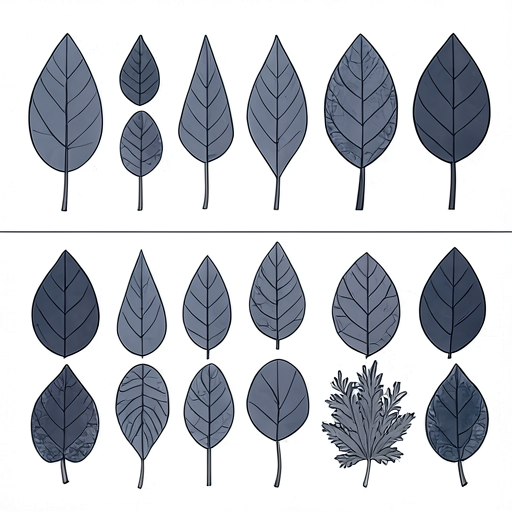
\includegraphics[width=0.95\textwidth]{img/analogia_exemplos_rotulados_folhas.png}\\
{\footnotesize\textbf{Supervisionado}\\ exemplos com rótulo}
\column{0.32\textwidth}
\centering
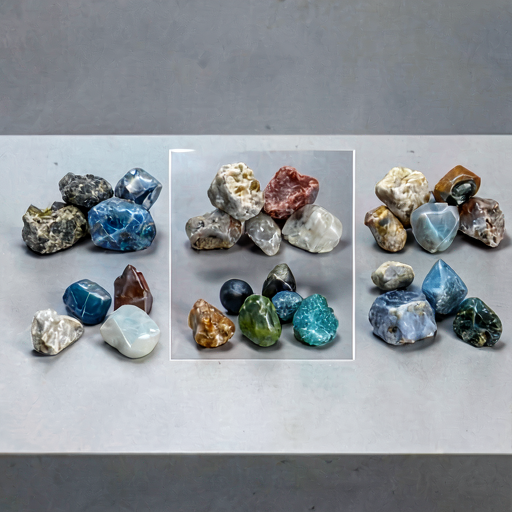
\includegraphics[width=0.95\textwidth]{img/analogia_amostras_agrupadas.png}\\
{\footnotesize\textbf{Não supervisionado}\\ estrutura sem rótulo}
\column{0.32\textwidth}
\centering
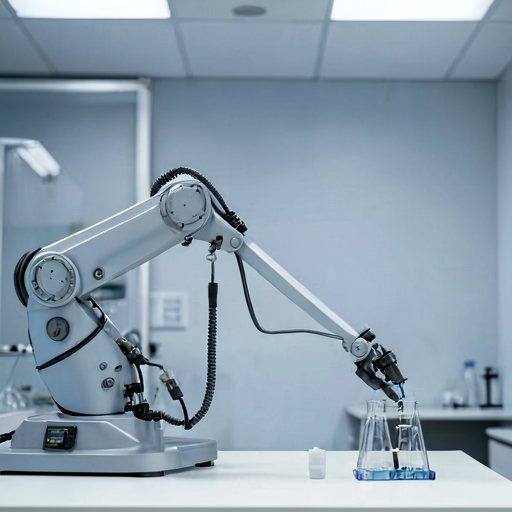
\includegraphics[width=0.95\textwidth]{img/analogia_braco_robotico_reforco.png}\\
{\footnotesize\textbf{Por reforço}\\ tentativa, erro e recompensa}
\end{columns}
\vspace{1mm}
{\scriptsize\captionof{figure}{Exemplos visuais dos três paradigmas: dados rotulados, amostras agrupadas por semelhança e um braço robótico que aprende por interação.}}
\end{frame}

\begin{frame}{Comparando os paradigmas}
\footnotesize
\begin{tabularx}{\textwidth}{@{}l X X X@{}}
\toprule
 & \textbf{Supervisionado} & \textbf{Não supervisionado} & \textbf{Reforço} \\
\midrule
Dados & pares $(x,y)$ & apenas $x$ & interação com o ambiente \\
Objetivo & prever $y$ & achar estrutura & maximizar recompensa \\
Exemplo & diagnóstico por imagem & segmentar clientes & robô que aprende a andar \\
\bottomrule
\end{tabularx}
\vspace{2mm}

\textbf{Dilema do reforço:} explorar ações novas ou aproveitar a melhor ação conhecida (\textit{exploration vs. exploitation}). É como escolher entre um restaurante novo e o seu favorito.
\end{frame}

\begin{frame}{Os modelos de linguagem usam qual paradigma?}
\begin{itemize}
 \item Pré-treino \textbf{autossupervisionado}: o rótulo é a próxima palavra do próprio texto.
 \item Ajuste fino \textbf{supervisionado} com exemplos de boas respostas.
 \item Alinhamento com \textbf{reforço} a partir de preferências humanas (RLHF).
\end{itemize}
\begin{reflexao}
Por que a autossupervisão permite treinar com bilhões de textos sem rotulagem manual?
\end{reflexao}
\end{frame}

%%%%%%%%%%%%%%%%%%%%%%%%%%%%%%%%%%%%%%%%
\section{Aprendizado Supervisionado}

\begin{frame}{Aprendizado supervisionado}
\begin{columns}[c]
\column{0.58\textwidth}
Dado um conjunto de exemplos
\[ \mathcal{D}=\{(x_i,y_i)\}_{i=1}^{m}, \]
queremos aprender uma função $h$ tal que $h(x)\approx y$ \textbf{também para dados novos}.
\begin{itemize}
 \item $x$: atributos (\textit{features}).
 \item $y$: rótulo ou valor alvo.
 \item Classificação: $y$ é uma categoria.
 \item Regressão: $y\in\mathbb{R}$.
\end{itemize}
\column{0.4\textwidth}
\centering
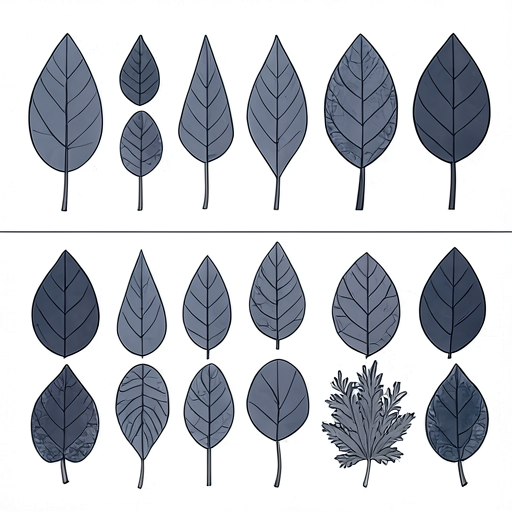
\includegraphics[width=\textwidth]{img/analogia_exemplos_rotulados_folhas.png}
{\scriptsize\captionof{figure}{Exemplos já rotulados por espécie.}}
\end{columns}
\begin{reflexao}
\small E se todas as folhas de uma espécie no treino vierem do mesmo jardim?
\end{reflexao}
\end{frame}

\begin{frame}{As peças do aprendizado}
\begin{itemize}
 \item \textbf{Modelo} $h_\theta$: família de funções com parâmetros $\theta$.
 \item \textbf{Perda} $\ell$: mede o erro de uma previsão.
 \item \textbf{Otimização}: escolhe $\theta$ que minimiza o risco empírico
\end{itemize}
\[ \hat{R}(\theta)=\frac{1}{m}\sum_{i=1}^{m}\ell\big(h_\theta(x_i),y_i\big). \]
\begin{itemize}
 \item \textbf{Avaliação}: mede o desempenho em dados que o modelo não viu.
\end{itemize}
\end{frame}

\begin{frame}{Fluxo de trabalho}
\centering
\begin{tikzpicture}[node distance=7mm, scale=1.15, transform shape]
  \node[caixa] (a) {Coletar e\\limpar};
  \node[caixa, right=of a] (b) {Dividir\\treino/teste};
  \node[caixa, right=of b] (c) {Treinar};
  \node[caixa, right=of c] (d) {Avaliar};
  \node[caixa, fill=verde!15, draw=verde, right=of d] (e) {Implantar};
  \draw[seta] (a)--(b); \draw[seta] (b)--(c); \draw[seta] (c)--(d); \draw[seta] (d)--(e);
  \draw[seta, laranja, dashed] (d.south) -- ++(0,-0.8) -| node[near start, below, text=laranja] {ajustar hiperparâmetros e dados} (c.south);
\end{tikzpicture}
\end{frame}

\begin{frame}{Classificação e regressão}
\centering
\begin{tikzpicture}
\begin{groupplot}[group style={group size=2 by 1, horizontal sep=14mm}, width=0.42\textwidth, height=0.32\textwidth, axis lines=left, xtick=\empty, ytick=\empty, xlabel={$x_1$}]
\nextgroupplot[title={Classificação}, ylabel={$x_2$}, xmin=0, xmax=6, ymin=0, ymax=6]
\addplot[only marks, mark=*, mark size=1.6pt, azul] coordinates {(1,1.2)(1.5,2.3)(2,1)(2.4,2)(1,3)(1.8,0.5)};
\addplot[only marks, mark=triangle*, mark size=2pt, laranja] coordinates {(4,4.5)(4.8,3.5)(3.5,5)(5,5.2)(4.4,2.8)(5.3,4.2)};
\addplot[thick, dashed, black, domain=0.8:5.5] {6.4-x};
\nextgroupplot[title={Regressão}, ylabel={$y$}, xmin=0, xmax=6, ymin=0, ymax=6]
\addplot[only marks, mark=*, mark size=1.6pt, azul] coordinates {(0.8,1.2)(1.5,2.1)(2.2,2.2)(3,3.4)(3.7,3.3)(4.4,4.6)(5.2,5)};
\addplot[thick, laranja, domain=0.4:5.6] {0.7+0.85*x};
\end{groupplot}
\end{tikzpicture}

\small A saída é uma \textbf{categoria} na classificação e um \textbf{número} na regressão.
\end{frame}

\begin{frame}{Treino e teste}
\centering
\begin{tikzpicture}
  \fill[azul!25] (0,0) rectangle (8,0.7); \node at (4,0.35) {\small Treino (80\%)};
  \fill[verde!30] (8,0) rectangle (10,0.7); \node at (9,0.35) {\small Teste (20\%)};
  \draw (0,0) rectangle (10,0.7);
\end{tikzpicture}
\begin{itemize}
 \item \textbf{Treino}: ajusta os parâmetros.
 \item \textbf{Teste}: estima o desempenho final, e deve ser usado uma única vez.
\end{itemize}
\end{frame}

\begin{frame}{Underfitting e overfitting}
\centering
\begin{tikzpicture}
\begin{groupplot}[group style={group size=3 by 1, horizontal sep=5mm}, width=0.33\textwidth, height=0.3\textwidth, xmin=0, xmax=6, ymin=-0.5, ymax=5.5, xtick=\empty, ytick=\empty, axis lines=left, title style={font=\footnotesize\bfseries}]
\nextgroupplot[title={Underfitting}]
\addplot[only marks, mark=*, mark size=1.4pt, azul] coordinates {(0.5,1.6)(1,2.3)(1.5,2.6)(2,3.9)(2.5,3.4)(3,4.6)(3.5,3.6)(4,3.2)(4.5,2.2)(5.5,0.7)};
\addplot[thick, vermelho, domain=0.3:5.7] {3.10455-0.10519*x};
\nextgroupplot[title={Bom ajuste}]
\addplot[only marks, mark=*, mark size=1.4pt, azul] coordinates {(0.5,1.6)(1,2.3)(1.5,2.6)(2,3.9)(2.5,3.4)(3,4.6)(3.5,3.6)(4,3.2)(4.5,2.2)(5.5,0.7)};
\addplot[thick, verde, domain=0.3:5.7] {0.24866+2.57118*x-0.45694*x^2};
\nextgroupplot[title={Overfitting}]
\addplot[only marks, mark=*, mark size=1.4pt, azul] coordinates {(0.5,1.6)(1,2.3)(1.5,2.6)(2,3.9)(2.5,3.4)(3,4.6)(3.5,3.6)(4,3.2)(4.5,2.2)(5.5,0.7)};
\addplot[thick, laranja, smooth, tension=0.6] coordinates {(0.5,1.6)(1,2.3)(1.5,2.6)(2,3.9)(2.5,3.4)(3,4.6)(3.5,3.6)(4,3.2)(4.5,2.2)(5.5,0.7)};
\end{groupplot}
\end{tikzpicture}
\captionof{figure}{Mesmos dados, três modelos: reta, parábola e curva que passa por todos os pontos.}
\end{frame}

\begin{frame}{Como diagnosticar}
\small
\begin{tabularx}{\textwidth}{@{}l c c X@{}}
\toprule
\textbf{Situação} & \textbf{Erro treino} & \textbf{Erro teste} & \textbf{O que fazer} \\
\midrule
Underfitting & alto & alto & modelo mais flexível, mais atributos \\
Bom ajuste & baixo & baixo & manter e testar \\
Overfitting & baixo & alto & mais dados, regularização, modelo mais simples \\
\bottomrule
\end{tabularx}
\end{frame}

\begin{frame}{Viés e variância}
\begin{columns}[c]
\column{0.5\textwidth}
\begin{tikzpicture}
\begin{axis}[width=\textwidth, height=0.8\textwidth, axis lines=left, xlabel={Complexidade do modelo}, ylabel={Erro}, xtick=\empty, ytick=\empty, legend pos=north west, legend style={font=\tiny, draw=none, fill=none}, ymin=0, ymax=3.2, xmin=0, xmax=6]
\addplot[thick, azul, domain=0.2:5.8] {2.6*exp(-0.6*x)+0.25};
\addplot[thick, laranja, domain=0.2:5.8] {2.6*exp(-0.6*x)+0.35+0.02*x^3};
\legend{Treino, Teste}
\end{axis}
\end{tikzpicture}
\column{0.48\textwidth}
\small
Erro esperado com perda quadrática:
\[ \text{viés}^2+\text{variância}+\text{ruído}. \]
\begin{itemize}
 \item Pouca complexidade: viés alto.
 \item Muita complexidade: variância alta.
 \item Buscamos o ponto intermediário.
\end{itemize}
\end{columns}
\end{frame}

\begin{frame}{Memorizar não é entender}
\textbf{Como evitar o overfitting}
\begin{itemize}
 \item Mais dados de boa qualidade.
 \item Modelo mais simples.
 \item Regularização.
 \item Cross-validation.
\end{itemize}
\begin{reflexao}
Um aluno que decorou a prova de 2023 está preparado para a de 2024?
\end{reflexao}
\end{frame}

%%%%%%%%%%%%%%%%%%%%%%%%%%%%%%%%%%%%%%%%
\section{Projeto de ML}

\begin{frame}{As oito etapas de um projeto}
\centering
\begin{tikzpicture}[etapa/.style={caixa, minimum width=2.05cm, minimum height=0.8cm}]
  \node[etapa] (n1) at (0,0)     {1. Problema};
  \node[etapa] (n2) at (2.5,0)   {2. Dados};
  \node[etapa] (n3) at (5.0,0)   {3. Exploração};
  \node[etapa] (n4) at (7.5,0)   {4. Preparação};
  \node[etapa] (n5) at (7.5,-2)  {5. Modelos};
  \node[etapa] (n6) at (5.0,-2)  {6. Ajuste};
  \node[etapa] (n7) at (2.5,-2)  {7. Apresentação};
  \node[etapa, fill=verde!15, draw=verde] (n8) at (0,-2) {8. Produção};
  \draw[seta] (n1) -- (n2);
  \draw[seta] (n2) -- (n3);
  \draw[seta] (n3) -- (n4);
  \draw[seta] (n4) -- (n5);
  \draw[seta] (n5) -- (n6);
  \draw[seta] (n6) -- (n7);
  \draw[seta] (n7) -- (n8);
  \draw[seta, laranja, dashed] (n8) -- node[left, font=\scriptsize, text=laranja] {monitorar} (n1);
\end{tikzpicture}

\vspace{4mm}\small O processo é iterativo: a monitoração em produção gera novos dados que reiniciam o ciclo.
\end{frame}

\begin{frame}{1. Problema e 2. Dados}
\begin{columns}[T]
\column{0.5\textwidth}
\textbf{Reflita sobre o problema}
\begin{itemize}
 \item Qual é o objetivo de negócio?
 \item Como a solução será usada?
 \item Como medir o sucesso?
 \item Existe uma linha de base simples?
\end{itemize}
\column{0.5\textwidth}
\textbf{Obtenha os dados}
\begin{itemize}
 \item Quais dados e em que volume?
 \item Há restrições legais e de privacidade?
 \item Separe o conjunto de teste agora e não o toque.
\end{itemize}
\end{columns}
\end{frame}

\begin{frame}{3. Exploração e 4. Preparação}
\begin{columns}[T]
\column{0.5\textwidth}
\textbf{Explore}
\begin{itemize}
 \item Trabalhe em uma cópia dos dados.
 \item Estude tipo, ausências e distribuição de cada atributo.
 \item Visualize e meça correlações.
\end{itemize}
\column{0.5\textwidth}
\textbf{Prepare}
\begin{itemize}
 \item Trate ausências e \textit{outliers}.
 \item Codifique categorias.
 \item Padronize atributos numéricos.
 \item Escreva funções reutilizáveis.
\end{itemize}
\end{columns}
\end{frame}

\begin{frame}{5. Modelos, 6. Ajuste e 7. Apresentação}
\begin{itemize}
 \item Treine modelos de famílias diferentes e compare por cross-validation.
 \item Ajuste os hiperparâmetros dos três a cinco melhores candidatos.
 \item Combine modelos (\textit{ensembles}) se houver ganho real.
 \item Documente suposições e limitações antes de apresentar.
\end{itemize}
\begin{atencao}
Não ajuste o modelo depois de olhar o erro no teste. Ele deixa de ser uma estimativa honesta.
\end{atencao}
\end{frame}

\begin{frame}{8. Produção}
\begin{itemize}
 \item Conecte o modelo às fontes de dados e escreva testes.
 \item Monitore o desempenho com dados reais.
 \item Verifique a qualidade das entradas (sensores com defeito, dados antigos).
 \item Retreine com dados novos para acompanhar mudanças no mundo (\textit{data drift}).
\end{itemize}
\end{frame}

\begin{frame}[fragile]{Vazamento de dados}
\begin{columns}[T]
\column{0.48\textwidth}
\textbf{Errado}: normalizar tudo antes de dividir.
\begin{lstlisting}
X = StandardScaler().fit_transform(X)
X_tr, X_te = train_test_split(X)
\end{lstlisting}
O teste influenciou a média e o desvio usados no treino.
\column{0.48\textwidth}
\textbf{Certo}: aprender a transformação só no treino.
\begin{lstlisting}
X_tr, X_te = train_test_split(X)
pipe = make_pipeline(
    StandardScaler(),
    LogisticRegression())
pipe.fit(X_tr, y_tr)
\end{lstlisting}
\end{columns}
\end{frame}

\begin{frame}{Algoritmos clássicos}
\footnotesize
\begin{tabularx}{\textwidth}{@{}l X X@{}}
\toprule
\textbf{Algoritmo} & \textbf{Ideia} & \textbf{Ponto de atenção} \\
\midrule
k-NN & classe dos $k$ vizinhos mais próximos & lento com muitos dados e sensível à escala \\
Árvore de decisão & perguntas sucessivas sobre atributos & tende ao overfitting \\
\textit{Random Forest} & muitas árvores votando & menos interpretável \\
Naive Bayes & probabilidades com atributos independentes & independência raramente vale \\
SVM & margem máxima entre classes & custo alto em bases grandes \\
Regressão logística & probabilidade por função sigmoide & fronteira linear \\
\bottomrule
\end{tabularx}
\end{frame}

\begin{frame}[fragile]{Exemplo completo com scikit-learn}
\begin{lstlisting}
from sklearn.datasets import load_breast_cancer
from sklearn.model_selection import train_test_split, GridSearchCV
from sklearn.pipeline import make_pipeline
from sklearn.preprocessing import StandardScaler
from sklearn.linear_model import LogisticRegression
from sklearn.metrics import classification_report

X, y = load_breast_cancer(return_X_y=True)
X_tr, X_te, y_tr, y_te = train_test_split(
    X, y, test_size=0.2, stratify=y, random_state=42)

pipe = make_pipeline(StandardScaler(),
                     LogisticRegression(max_iter=1000))
grid = GridSearchCV(
    pipe, {"logisticregression__C": [0.01, 0.1, 1, 10]}, cv=5)
grid.fit(X_tr, y_tr)
print(classification_report(y_te, grid.predict(X_te)))
\end{lstlisting}
\end{frame}

%%%%%%%%%%%%%%%%%%%%%%%%%%%%%%%%%%%%%%%%
\section{Seleção e Teste}

\begin{frame}{Seleção de modelos}
\begin{itemize}
 \item \textbf{Seleção}: escolher a família de hipóteses (árvores, redes, regressão).
 \item \textbf{Otimização}: achar a melhor hipótese dentro da família escolhida.
 \item O desafio é equilibrar underfitting e overfitting.
\end{itemize}
\vspace{2mm}
\begin{tabularx}{\textwidth}{@{}l X X@{}}
\toprule
 & \textbf{Parâmetros} & \textbf{Hiperparâmetros} \\
\midrule
Quem define & o algoritmo, ao treinar & a pessoa, antes de treinar \\
Exemplos & pesos, coeficientes & $k$ do k-NN, profundidade, $\lambda$ \\
\bottomrule
\end{tabularx}
\end{frame}

\begin{frame}{Cross-validation com $k$ partições}
\centering
\begin{tikzpicture}[x=1.7cm]
  \foreach \r in {1,...,5} {
    \foreach \c in {1,...,5} {
      \ifnum\r=\c
        \fill[laranja!45] (\c-1,-\r*0.55) rectangle (\c,-\r*0.55+0.45);
      \else
        \fill[azul!25] (\c-1,-\r*0.55) rectangle (\c,-\r*0.55+0.45);
      \fi
      \draw (\c-1,-\r*0.55) rectangle (\c,-\r*0.55+0.45);
    }
    \node[anchor=east, font=\scriptsize] at (-0.1,-\r*0.55+0.22) {Rodada \r};
  }
  \fill[azul!25] (0,-4) rectangle (0.4,-3.75); \node[anchor=west, font=\scriptsize] at (0.45,-3.87) {treino};
  \fill[laranja!45] (1.5,-4) rectangle (1.9,-3.75); \node[anchor=west, font=\scriptsize] at (1.95,-3.87) {teste};
\end{tikzpicture}

\begin{itemize}\small
 \item Cada partição serve uma vez como teste.
 \item O resultado é a média das $k$ notas, com seu desvio padrão.
\end{itemize}
\end{frame}

\begin{frame}{Cross-validation: um exemplo numérico}
Cinco rodadas, acurácias de teste: $0{,}84$, $0{,}88$, $0{,}80$, $0{,}86$, $0{,}82$.
\[ \bar{a}=0{,}84, \qquad s=\sqrt{\frac{0+0{,}0016+0{,}0016+0{,}0004+0{,}0004}{4}}\approx 0{,}032. \]
Relatamos $0{,}84\pm0{,}03$. A cross-validation reduz a variância da estimativa de desempenho, porque não depende de uma única divisão.
\begin{reflexao}
\small Dados de séries temporais podem ser embaralhados antes da divisão? Por quê?
\end{reflexao}
\end{frame}

\begin{frame}{Curvas de aprendizado}
\centering
\begin{tikzpicture}
\begin{groupplot}[group style={group size=2 by 1, horizontal sep=10mm}, width=0.42\textwidth, height=0.32\textwidth, axis lines=left, xtick=\empty, ytick=\empty, xlabel={Tamanho do treino}, ylabel={Erro}, ymin=0, ymax=1, xmin=0, xmax=5, title style={font=\footnotesize\bfseries}]
\nextgroupplot[title={Viés alto}]
\addplot[thick, azul, domain=0.3:5] {0.55+0.35*exp(-1.2*x)};
\addplot[thick, laranja, domain=0.3:5] {0.55-0.05*exp(-1.2*x)+0.0};
\nextgroupplot[title={Variância alta}]
\addplot[thick, azul, domain=0.3:5] {0.02+0.3*exp(-1.0*x)};
\addplot[thick, laranja, domain=0.3:5] {0.55*exp(-0.35*x)+0.2};
\end{groupplot}
\end{tikzpicture}

{\scriptsize\textcolor{azul}{azul}: erro de treino. \textcolor{laranja}{laranja}: erro de teste (curvas ilustrativas).}

\small No viés alto, mais dados não ajudam. Na variância alta, mais dados ajudam.
\end{frame}

\begin{frame}{Busca de hiperparâmetros}
\centering
\begin{tikzpicture}[scale=0.9]
  \draw (0,0) rectangle (3,3); \node[above] at (1.5,3) {\footnotesize Grid};
  \foreach \x in {0.5,1.5,2.5} \foreach \y in {0.5,1.5,2.5} \fill[azul] (\x,\y) circle (2pt);
  \draw (4.5,0) rectangle (7.5,3); \node[above] at (6,3) {\footnotesize Random};
  \foreach \x/\y in {0.4/2.6,1.1/0.7,1.6/1.9,2.2/0.3,2.7/2.2,0.8/1.3,1.9/2.8,2.5/1.1,0.3/0.4} \fill[laranja] ({4.5+\x},\y) circle (2pt);
  \node[font=\scriptsize] at (1.5,-0.35) {$\lambda$};
\end{tikzpicture}

\small Com a mesma quantidade de testes, a random search explora mais valores distintos de cada hiperparâmetro. A otimização bayesiana usa os resultados anteriores para escolher o próximo teste.
\end{frame}

%%%%%%%%%%%%%%%%%%%%%%%%%%%%%%%%%%%%%%%%
\section{Matriz de Confusão}

\begin{frame}{Matriz de confusão}
\centering
\begin{tikzpicture}[every node/.style={font=\footnotesize, align=center}]
  \node at (3.0,3.2) {\textbf{Previsto}};
  \node[rotate=90] at (-0.9,1.1) {\textbf{Real}};
  \node at (1.3,2.6) {Positivo}; \node at (3.7,2.6) {Negativo};
  \node[anchor=east] at (0,1.8) {Positivo}; \node[anchor=east] at (0,0.4) {Negativo};
  \fill[verde!25] (0,1.2) rectangle (2.6,2.4); \node at (1.3,1.8) {Verdadeiro Positivo\\(VP)};
  \fill[vermelho!20] (2.6,1.2) rectangle (4.8,2.4); \node at (3.7,1.8) {Falso Negativo\\(FN)};
  \fill[vermelho!20] (0,0) rectangle (2.6,1.2); \node at (1.3,0.6) {Falso Positivo\\(FP)};
  \fill[verde!25] (2.6,0) rectangle (4.8,1.2); \node at (3.7,0.6) {Verdadeiro Negativo\\(VN)};
  \draw (0,0) rectangle (4.8,2.4); \draw (2.6,0)--(2.6,2.4); \draw (0,1.2)--(4.8,1.2);
\end{tikzpicture}

\small A diagonal mostra os acertos. Fora dela estão os dois tipos de erro.
\end{frame}

\begin{frame}{VP, FN, FP, VN e suas equações}
\begin{itemize}
 \item \textbf{VP (verdadeiro positivo)}: positivo previsto e real positivo.
 \item \textbf{FN (falso negativo)}: negativo previsto, mas real positivo.
 \item \textbf{FP (falso positivo)}: positivo previsto, mas real negativo.
 \item \textbf{VN (verdadeiro negativo)}: negativo previsto e real negativo.
\end{itemize}
\vspace{2mm}
\begin{align*}
\text{Acurácia} &= \frac{VP+VN}{VP+FN+FP+VN} \\
\text{Precisão} &= \frac{VP}{VP+FP} \\
\text{Recall} &= \frac{VP}{VP+FN} \\
F_1 &= \frac{2\cdot\text{Precisão}\cdot\text{Recall}}{\text{Precisão}+\text{Recall}}
\end{align*}
\end{frame}

\begin{frame}{Exemplo: filtro de spam}
\centering
\begin{tabular}{@{}lcc@{}}
\toprule
 & \textbf{Previsto spam} & \textbf{Previsto não spam} \\
\midrule
\textbf{Real spam} & 50 (VP) & 10 (FN) \\
\textbf{Real não spam} & 5 (FP) & 100 (VN) \\
\bottomrule
\end{tabular}

\vspace{3mm}
\begin{tabularx}{\textwidth}{@{}l X c@{}}
\toprule
\textbf{Métrica} & \textbf{Pergunta que responde} & \textbf{Valor} \\
\midrule
Acurácia & quanto acertamos no total? & $\frac{150}{165}\approx 90{,}9\%$ \\
Precisão & dos que previmos spam, quantos eram? & $\frac{50}{55}\approx 90{,}9\%$ \\
\textit{Recall} & dos spams reais, quantos achamos? & $\frac{50}{60}\approx 83{,}3\%$ \\
F1 & equilíbrio entre precisão e \textit{recall} & $\frac{2\cdot50}{2\cdot50+5+10}\approx 0{,}87$ \\
\bottomrule
\end{tabularx}
\end{frame}

\begin{frame}{O paradoxo da acurácia}
Em $1000$ pacientes, apenas $10$ têm a doença. Um modelo que responde sempre ``saudável'' obtém:
\[ \text{acurácia}=\frac{990}{1000}=99\%, \qquad \text{\textit{recall}}=\frac{0}{10}=0\%. \]
\begin{reflexao}
Esse modelo é útil? Qual métrica revela o problema?
\end{reflexao}
\small Com classes desbalanceadas, use \textit{recall}, precisão, F1 e a matriz de confusão.
\end{frame}

\begin{frame}{Qual erro custa mais?}
\small
\begin{tabularx}{\textwidth}{@{}l X X@{}}
\toprule
\textbf{Cenário} & \textbf{Erro mais grave} & \textbf{Priorizar} \\
\midrule
Triagem de câncer & falso negativo (doença não detectada) & \textit{recall} \\
Filtro de spam & falso positivo (e-mail importante perdido) & precisão \\
Detecção de fraude & depende do custo da fraude e da revisão & ambos, via F1 ou custo \\
\bottomrule
\end{tabularx}

\vspace{2mm}
O limiar de decisão controla essa troca. Reduzir o limiar aumenta o \textit{recall} e diminui a precisão.
\end{frame}

\begin{frame}{Classificação multiclasse}
\begin{columns}[c]
\column{0.5\textwidth}
\centering
\begin{tikzpicture}[every node/.style={font=\footnotesize}]
  \foreach \i/\j/\v/\p/\t in {0/0/45/90/white,0/1/3/8/black,0/2/2/6/black,1/0/4/10/black,1/1/38/80/white,1/2/8/18/black,2/0/1/4/black,2/1/6/14/black,2/2/43/86/white} {
    \fill[azul!\p] (\j*0.9,-\i*0.9) rectangle (\j*0.9+0.9,-\i*0.9-0.9);
    \node[text=\t] at (\j*0.9+0.45,-\i*0.9-0.45) {\v};
  }
  \foreach \l/\k in {A/0,B/1,C/2} {
    \node at (\k*0.9+0.45,0.3) {\l}; \node at (-0.3,-\k*0.9-0.45) {\l};
  }
  \node at (1.35,0.7) {Previsto}; \node[rotate=90] at (-0.8,-1.35) {Real};
\end{tikzpicture}
\column{0.48\textwidth}
\footnotesize
\begin{tabular}{@{}lccc@{}}
\toprule
 & Prec. & \textit{Recall} & F1 \\
\midrule
A & 0,90 & 0,90 & 0,90 \\
B & 0,81 & 0,76 & 0,78 \\
C & 0,81 & 0,86 & 0,84 \\
\bottomrule
\end{tabular}

\vspace{2mm}
Acurácia: $126/150=84\%$. Média macro do F1: $0{,}84$.
\end{columns}
\vspace{1mm}
\small Cada linha soma os exemplos reais da classe. A classe B é a mais confundida.
\end{frame}

\begin{frame}{Exercício}
Um detector de fraude produziu $VP=30$, $FN=20$, $FP=10$ e $VN=940$.

Calcule acurácia, precisão, \textit{recall} e F1.

\pause
\vspace{2mm}
\begin{block}{Resposta}
Acurácia $=970/1000=97\%$. Precisão $=30/40=0{,}75$. \textit{Recall} $=30/50=0{,}60$. F1 $=60/90\approx0{,}67$.
\end{block}
\small A acurácia alta esconde que $40\%$ das fraudes passam despercebidas.
\end{frame}

%%%%%%%%%%%%%%%%%%%%%%%%%%%%%%%%%%%%%%%%
\section{Regressão}

\begin{frame}{Regressão linear simples}
\begin{columns}[c]
\column{0.5\textwidth}
\[ y=\beta_0+\beta_1x+\varepsilon \]
\begin{itemize}
 \item $\beta_0$: intercepto.
 \item $\beta_1$: variação esperada em $y$ para cada unidade de $x$.
 \item $\varepsilon$: erro aleatório.
\end{itemize}
Os coeficientes minimizam a soma dos quadrados dos resíduos (mínimos quadrados).
\column{0.5\textwidth}
\begin{tikzpicture}
\begin{axis}[width=\textwidth, height=0.85\textwidth, axis lines=left, xlabel={$x$}, ylabel={$y$}, xmin=0, xmax=6, ymin=0, ymax=7, xtick={1,...,5}, ytick={1,...,6}]
\addplot[only marks, mark=*, azul] coordinates {(1,2)(2,3)(3,5)(4,4)(5,6)};
\addplot[thick, laranja, domain=0.3:5.7] {1.3+0.9*x};
\draw[vermelho, dashed] (axis cs:1,2) -- (axis cs:1,2.2);
\draw[vermelho, dashed] (axis cs:2,3) -- (axis cs:2,3.1);
\draw[vermelho, dashed] (axis cs:3,5) -- (axis cs:3,4.0);
\draw[vermelho, dashed] (axis cs:4,4) -- (axis cs:4,4.9);
\draw[vermelho, dashed] (axis cs:5,6) -- (axis cs:5,5.8);
\end{axis}
\end{tikzpicture}
\end{columns}
\end{frame}

\begin{frame}{Exemplo resolvido}
Dados $(x,y)$: $(1,2),(2,3),(3,5),(4,4),(5,6)$. Médias: $\bar{x}=3$ e $\bar{y}=4$.
\[ \hat\beta_1=\frac{\sum(x_i-\bar{x})(y_i-\bar{y})}{\sum(x_i-\bar{x})^2}=\frac{9}{10}=0{,}9, \qquad \hat\beta_0=\bar{y}-\hat\beta_1\bar{x}=1{,}3. \]
\small
\begin{tabular}{@{}c|ccccc@{}}
\toprule
$x$ & 1 & 2 & 3 & 4 & 5 \\
$y$ & 2 & 3 & 5 & 4 & 6 \\
$\hat{y}$ & 2,2 & 3,1 & 4,0 & 4,9 & 5,8 \\
resíduo & $-0{,}2$ & $-0{,}1$ & $1{,}0$ & $-0{,}9$ & $0{,}2$ \\
\bottomrule
\end{tabular}
\end{frame}

\begin{frame}{Métricas de regressão}
\small
\begin{tabularx}{\textwidth}{@{}l c X@{}}
\toprule
\textbf{Métrica} & \textbf{Fórmula} & \textbf{No exemplo} \\
\midrule
MSE & $\frac{1}{n}\sum(y_i-\hat{y}_i)^2$ & $1{,}90/5=0{,}38$ \\
RMSE & $\sqrt{\text{MSE}}$ & $0{,}62$, na unidade de $y$ \\
MAE & $\frac{1}{n}\sum|y_i-\hat{y}_i|$ & $2{,}4/5=0{,}48$ \\
$R^2$ & $1-\frac{\sum(y_i-\hat{y}_i)^2}{\sum(y_i-\bar{y})^2}$ & $1-\frac{1{,}9}{10}=0{,}81$ \\
\bottomrule
\end{tabularx}

\vspace{2mm}
\begin{itemize}\small
 \item O MSE pune erros grandes mais do que o MAE.
 \item $R^2$ pode ser \textbf{negativo} em dados de teste, quando o modelo é pior que a média.
 \item $R^2$ ajustado penaliza atributos que não ajudam.
\end{itemize}
\end{frame}

\begin{frame}{Regressão múltipla}
\[ y=\beta_0+\beta_1x_1+\cdots+\beta_px_p+\varepsilon \quad\Longleftrightarrow\quad \mathbf{y}=\mathbf{X}\boldsymbol\beta+\boldsymbol\varepsilon. \]
Com $\mathbf{X}\in\mathbb{R}^{n\times(p+1)}$ (primeira coluna de uns), a solução de mínimos quadrados é
\[ \hat{\boldsymbol\beta}=(\mathbf{X}^\top\mathbf{X})^{-1}\mathbf{X}^\top\mathbf{y}. \]
Cada $\beta_j$ mede o efeito de $x_j$ \textbf{mantendo os demais fixos}. Exemplo: o preço de um imóvel cresce $\beta_1$ por metro quadrado, com o número de quartos constante.
\end{frame}

\begin{frame}{Regressão polinomial}
\begin{columns}[c]
\column{0.5\textwidth}
\[ y=\beta_0+\beta_1x+\beta_2x^2+\cdots+\beta_dx^d \]
O modelo é \textbf{linear nos coeficientes}, mesmo com curva em $x$. Por isso os mesmos mínimos quadrados se aplicam.

\vspace{2mm}
\small Na figura de underfitting e overfitting, a reta tem $\text{SSE}=11{,}9$ e a parábola $1{,}3$.
\column{0.5\textwidth}
\begin{tikzpicture}
\begin{axis}[width=\textwidth, height=0.85\textwidth, axis lines=left, xtick=\empty, ytick=\empty, xlabel={$x$}, ylabel={$y$}, ymin=-0.5, ymax=5.5, xmin=0, xmax=6]
\addplot[only marks, mark=*, azul, mark size=1.4pt] coordinates {(0.5,1.6)(1,2.3)(1.5,2.6)(2,3.9)(2.5,3.4)(3,4.6)(3.5,3.6)(4,3.2)(4.5,2.2)(5.5,0.7)};
\addplot[thick, vermelho, domain=0.3:5.7] {3.10455-0.10519*x};
\addplot[thick, verde, domain=0.3:5.7] {0.24866+2.57118*x-0.45694*x^2};
\end{axis}
\end{tikzpicture}
\end{columns}
\end{frame}

\begin{frame}{Regularização}
Penaliza coeficientes grandes para reduzir a variância:
\begin{align*}
\text{Ridge (L2):}&\quad \|\mathbf{y}-\mathbf{X}\boldsymbol\beta\|^2+\lambda\|\boldsymbol\beta\|_2^2\\
\text{Lasso (L1):}&\quad \|\mathbf{y}-\mathbf{X}\boldsymbol\beta\|^2+\lambda\|\boldsymbol\beta\|_1
\end{align*}
\begin{itemize}
 \item Ridge encolhe todos os coeficientes.
 \item Lasso pode zerar coeficientes e, assim, selecionar atributos.
 \item Padronize os atributos antes e não penalize o intercepto.
 \item Escolha $\lambda$ por cross-validation.
\end{itemize}
\end{frame}

\begin{frame}{Regressão logística}
\begin{columns}[c]
\column{0.5\textwidth}
Apesar do nome, é um \textbf{classificador}:
\[ P(y=1\mid\mathbf{x})=\sigma(z),\quad z=\mathbf{w}^\top\mathbf{x}+b. \]
\[ \sigma(z)=\frac{1}{1+e^{-z}}. \]
Prevemos a classe 1 quando $P\ge 0{,}5$, isto é, quando $\mathbf{w}^\top\mathbf{x}+b\ge0$. A perda é a entropia cruzada.
\column{0.5\textwidth}
\begin{tikzpicture}
\begin{axis}[width=\textwidth, height=0.8\textwidth, axis lines=left, xlabel={$z$}, ylabel={$\sigma(z)$}, ymin=0, ymax=1.1, ytick={0,0.5,1}, domain=-6:6]
\addplot[thick, laranja, samples=60] {1/(1+exp(-x))};
\addplot[dashed, gray, domain=-6:6] {0.5};
\end{axis}
\end{tikzpicture}
\end{columns}
\end{frame}

\begin{frame}{Suposições da regressão linear}
\footnotesize
\begin{tabularx}{\textwidth}{@{}l X X@{}}
\toprule
\textbf{Suposição} & \textbf{Como verificar} & \textbf{Possível remédio} \\
\midrule
Linearidade (nos parâmetros) & resíduos contra valores previstos & transformar variáveis ou incluir termos polinomiais \\
\bottomrule
\end{tabularx}

\vspace{1mm}
\centering
\begin{tikzpicture}
\begin{groupplot}[group style={group size=2 by 2, horizontal sep=12mm, vertical sep=6mm}, width=0.42\textwidth, height=0.2\textwidth, xtick=\empty, ytick=\empty, axis lines=left, xmin=0, xmax=6, title style={font=\scriptsize\bfseries}, label style={font=\tiny}]
\nextgroupplot[title={\textcolor{verde}{OK}: relação linear}, ymin=0, ymax=4, ylabel={$y$}]
\addplot[only marks, mark=*, mark size=1.1pt, azul] coordinates {(0,1.2)(1,1.2)(2,2.1)(3,2.8)(4,2.8)(5,3.6)(6,3.9)};
\addplot[thick, vermelho, domain=0:6] {1+0.5*x};
\nextgroupplot[title={\textcolor{vermelho}{Não OK}: relação curva}, ymin=0, ymax=4]
\addplot[only marks, mark=*, mark size=1.1pt, azul] coordinates {(0,2.75)(1,1.5)(2,0.75)(3,0.5)(4,0.75)(5,1.5)(6,2.75)};
\addplot[thick, vermelho, domain=0:6] {1.4};
\nextgroupplot[ymin=-1.5, ymax=1.5, ylabel={resíduo}, xlabel={$x$}]
\addplot[dashed, gray, domain=0:6] {0};
\addplot[only marks, mark=*, mark size=1.1pt, vermelho] coordinates {(0,0.2)(1,-0.3)(2,0.1)(3,0.3)(4,-0.2)(5,0.1)(6,-0.1)};
\nextgroupplot[ymin=-1.5, ymax=1.5, xlabel={$x$}]
\addplot[dashed, gray, domain=0:6] {0};
\addplot[only marks, mark=*, mark size=1.1pt, vermelho] coordinates {(0,1.35)(1,0.1)(2,-0.65)(3,-0.9)(4,-0.65)(5,0.1)(6,1.35)};
\end{groupplot}
\end{tikzpicture}

\small Esquerda: os resíduos são aleatórios em torno de zero. Direita: os resíduos formam uma curva em U, indicando não linearidade.
\end{frame}



\begin{frame}{Exercício}
Ajuste uma reta aos pontos $(1,2),(2,3),(3,5),(4,6)$ e preveja $y$ para $x=5$.

\pause
\begin{block}{Resposta}
$\bar{x}=2{,}5$, $\bar{y}=4$, $\hat\beta_1=7/5=1{,}4$, $\hat\beta_0=0{,}5$. Previsão: $\hat{y}(5)=7{,}5$. Os resíduos são $0{,}1$, $-0{,}3$, $0{,}3$ e $-0{,}1$, logo $\text{SSE}=0{,}2$ e $R^2=1-0{,}2/10=0{,}98$.
\end{block}
\end{frame}

%%%%%%%%%%%%%%%%%%%%%%%%%%%%%%%%%%%%%%%%
\section{Redes Neurais}

\begin{frame}{Do neurônio biológico ao artificial}
\centering
\begin{tikzpicture}[scale=0.95]
  % neurônio biológico
  \node[circle, draw=azul, fill=azul!15, minimum size=1.0cm] (soma) at (0,0) {};
  \foreach \a in {120,150,180,210,240} {
    \draw[azul!80!black, thick] (soma) -- ++(\a:1.1) -- ++({\a+25}:0.5);
  }
  \draw[azul!80!black, very thick] (soma) -- (3.2,0) -- ++(0.9,0.3);
  \draw[azul!80!black, thick] (3.2,0) -- ++(0.9,-0.3);
  \node[font=\scriptsize] at (-1.6,1.3) {dendritos};
  \node[font=\scriptsize] at (0,-0.85) {corpo celular};
  \node[font=\scriptsize] at (1.8,0.3) {axônio};
  \node[font=\scriptsize] at (3.9,0.8) {sinapses};
  % neurônio artificial
  \begin{scope}[xshift=6.3cm]
    \node[neuronio] (x1) at (0,0.9) {}; \node[left] at (x1) {\scriptsize $x_1$};
    \node[neuronio] (x2) at (0,0) {}; \node[left] at (x2) {\scriptsize $x_2$};
    \node[neuronio] (x3) at (0,-0.9) {}; \node[left] at (x3) {\scriptsize $x_3$};
    \node[circle, draw=laranja, fill=laranja!15, minimum size=0.9cm] (n) at (1.8,0) {$\sum\varphi$};
    \draw[seta] (x1) -- node[above, font=\tiny] {$w_1$} (n);
    \draw[seta] (x2) -- node[above, font=\tiny] {$w_2$} (n);
    \draw[seta] (x3) -- node[below, font=\tiny] {$w_3$} (n);
    \draw[seta] (n) -- ++(1.0,0) node[right, font=\scriptsize] {$y$};
  \end{scope}
\end{tikzpicture}

\small O neurônio artificial calcula $y=\varphi(\mathbf{w}^\top\mathbf{x}+b)$. A analogia biológica é inspiração e não um modelo fiel do cérebro.
\end{frame}

\begin{frame}{Neurônio biológico e artificial}
\small
\begin{tabularx}{\textwidth}{@{}l X X@{}}
\toprule
 & \textbf{Biológico} & \textbf{Artificial} \\
\midrule
Entrada & sinais nas sinapses & vetor $\mathbf{x}$ \\
Força da conexão & eficácia sináptica & peso $w_i$ \\
Disparo & potencial passa de um limiar & função de ativação $\varphi$ \\
Escala & cerca de $10^{11}$ neurônios, até $10^4$ conexões cada & de milhares a bilhões de parâmetros \\
\bottomrule
\end{tabularx}
\end{frame}

\begin{frame}{Funções de ativação}
\centering
\begin{tikzpicture}
\begin{groupplot}[group style={group size=2 by 2, horizontal sep=14mm, vertical sep=10mm}, width=0.36\textwidth, height=0.24\textwidth, axis lines=middle, xtick=\empty, ytick=\empty, xmin=-3, xmax=3, ymin=-1.3, ymax=1.5, title style={font=\footnotesize\bfseries}]
\nextgroupplot[title={Degrau}]
\addplot[thick, azul, domain=-3:-0.01] {0}; \addplot[thick, azul, domain=0:3] {1};
\nextgroupplot[title={Sigmoide}]
\addplot[thick, laranja, domain=-3:3, samples=50] {1/(1+exp(-2*x))};
\nextgroupplot[title={Tanh}]
\addplot[thick, verde, domain=-3:3, samples=50] {tanh(x)};
\nextgroupplot[title={ReLU}]
\addplot[thick, vermelho, domain=-3:3] {max(0,x)};
\end{groupplot}
\end{tikzpicture}
\end{frame}

\begin{frame}{Por que a não linearidade importa}
Sem ativação não linear, camadas empilhadas colapsam em uma só:
\[ W_2(W_1\mathbf{x}+\mathbf{b}_1)+\mathbf{b}_2=(W_2W_1)\mathbf{x}+(W_2\mathbf{b}_1+\mathbf{b}_2). \]
\small
\begin{tabularx}{\textwidth}{@{}l X X@{}}
\toprule
\textbf{Função} & \textbf{Uso típico} & \textbf{Observação} \\
\midrule
Sigmoide & saída binária & satura e atenua gradientes \\
Tanh & camadas ocultas antigas & centrada em zero \\
ReLU & camadas ocultas modernas & simples e rápida \\
Softmax & saída multiclasse & produz probabilidades \\
\bottomrule
\end{tabularx}
\end{frame}

\begin{frame}{O Perceptron}
\begin{columns}[c]
\column{0.5\textwidth}
Proposto por Rosenblatt (1958). Sobre o modelo de McCulloch e Pitts (1943), ele aprende os pesos:
\[ \hat{y}=\begin{cases}1,& \mathbf{w}^\top\mathbf{x}+b\ge0\\0,&\text{caso contrário.}\end{cases} \]
Geometricamente, a equação $\mathbf{w}^\top\mathbf{x}+b=0$ é uma reta que separa as classes.
\column{0.5\textwidth}
\begin{tikzpicture}
\begin{axis}[width=\textwidth, height=0.9\textwidth, axis lines=left, xtick=\empty, ytick=\empty, xlabel={$x_1$}, ylabel={$x_2$}, xmin=0, xmax=5, ymin=0, ymax=5]
\addplot[only marks, mark=*, azul] coordinates {(0.8,1)(1.4,2)(1,3)(2,0.8)(0.6,2.2)};
\addplot[only marks, mark=triangle*, laranja, mark size=2.2pt] coordinates {(3.5,3.8)(4.2,2.6)(3,4.4)(4.5,4.3)(3.8,3)};
\addplot[thick, black, domain=0.5:4.8] {5.4-x};
\draw[-{Stealth}, thick, vermelho] (axis cs:2.7,2.7) -- (axis cs:3.4,3.4) node[right, font=\scriptsize] {$\mathbf{w}$};
\end{axis}
\end{tikzpicture}
\end{columns}
\end{frame}

\begin{frame}{OR e AND com um neurônio}
Com $u=w_1x_1+w_2x_2+b$ e saída $1$ se $u\ge0$:
\begin{center}
\begin{tabular}{@{}cc|cc|cc@{}}
\toprule
$x_1$ & $x_2$ & \multicolumn{2}{c|}{OR: $w=(1,1),\ b=-0{,}5$} & \multicolumn{2}{c}{AND: $w=(1,1),\ b=-1{,}5$} \\
 & & $u$ & $y$ & $u$ & $y$ \\
\midrule
0 & 0 & $-0{,}5$ & 0 & $-1{,}5$ & 0 \\
0 & 1 & $0{,}5$ & 1 & $-0{,}5$ & 0 \\
1 & 0 & $0{,}5$ & 1 & $-0{,}5$ & 0 \\
1 & 1 & $1{,}5$ & 1 & $0{,}5$ & 1 \\
\bottomrule
\end{tabular}
\end{center}
\small O viés $b$ desloca a reta e faz o papel do antigo limiar $\theta=-b$.
\end{frame}

\begin{frame}{Regra de aprendizagem do Perceptron}
Para cada exemplo $(\mathbf{x},y)$ com previsão $\hat{y}$:
\[ \mathbf{w}\leftarrow\mathbf{w}+\eta\,(y-\hat{y})\,\mathbf{x}, \qquad b\leftarrow b+\eta\,(y-\hat{y}). \]
\begin{itemize}
 \item Se acertou, nada muda.
 \item Se errou, a reta se move em direção ao exemplo mal classificado.
 \item Se os dados são linearmente separáveis, o algoritmo converge em um número finito de passos.
\end{itemize}
\end{frame}

\begin{frame}{Exemplo resolvido: aprendendo AND}
Início: $w_1=w_2=0{,}2$, $b=-0{,}5$ e $\eta=0{,}1$.
\footnotesize
\begin{center}
\begin{tabular}{@{}cc c c c c c@{}}
\toprule
$x_1$ & $x_2$ & alvo & $u$ & $\hat{y}$ & erro & novos $w$ e $b$ \\
\midrule
0 & 0 & 0 & $-0{,}5$ & 0 & 0 & sem mudança \\
0 & 1 & 0 & $-0{,}3$ & 0 & 0 & sem mudança \\
1 & 0 & 0 & $-0{,}3$ & 0 & 0 & sem mudança \\
1 & 1 & 1 & $-0{,}1$ & 0 & $+1$ & $w_1=w_2=0{,}3$, $b=-0{,}4$ \\
\midrule
1 & 1 & 1 & $0{,}2$ & 1 & 0 & convergiu \\
\bottomrule
\end{tabular}
\end{center}
\small Na segunda passada, os quatro exemplos já são classificados corretamente.
\end{frame}

\begin{frame}{O problema do XOR}
\begin{columns}[c]
\column{0.45\textwidth}
\begin{tikzpicture}
\begin{axis}[width=\textwidth, height=\textwidth, axis lines=left, xlabel={$x_1$}, ylabel={$x_2$}, xmin=-0.4, xmax=1.4, ymin=-0.4, ymax=1.4, xtick={0,1}, ytick={0,1}]
\addplot[only marks, mark=*, azul, mark size=3pt] coordinates {(0,0)(1,1)};
\addplot[only marks, mark=triangle*, laranja, mark size=3.5pt] coordinates {(0,1)(1,0)};
\end{axis}
\end{tikzpicture}
\column{0.52\textwidth}
Nenhuma reta separa as classes. Por contradição, seriam necessárias:
\begin{itemize}\small
 \item $b<0$ e $w_1+w_2+b<0$,
 \item $w_1+b\ge0$ e $w_2+b\ge0$.
\end{itemize}
\small Somando as duas últimas: $w_1+w_2+2b\ge0$, logo $w_1+w_2+b\ge -b>0$. Isso contradiz a segunda desigualdade da primeira linha.

\vspace{1mm}
Minsky e Papert (1969) apontaram esse limite.
\end{columns}
\end{frame}

\begin{frame}{Duas camadas resolvem o XOR}
\centering
\begin{tikzpicture}[x=2.3cm, y=1.3cm]
  \node[neuronio] (a) at (0,0.6) {$x_1$}; \node[neuronio] (b) at (0,-0.6) {$x_2$};
  \node[neuronio, fill=laranja!15] (h1) at (1,0.6) {\scriptsize OR}; \node[neuronio, fill=laranja!15] (h2) at (1,-0.6) {\scriptsize NAND};
  \node[neuronio, fill=verde!20] (o) at (2,0) {\scriptsize AND};
  \draw[seta] (a)--(h1); \draw[seta] (b)--(h1); \draw[seta] (a)--(h2); \draw[seta] (b)--(h2);
  \draw[seta] (h1)--(o); \draw[seta] (h2)--(o); \draw[seta] (o)--++(0.6,0) node[right] {$y$};
\end{tikzpicture}

\vspace{4mm}\footnotesize
\begin{tabular}{@{}lll@{}}
\toprule
Neurônio & Pesos & Viés \\
\midrule
OR & $(1,1)$ & $-0{,}5$ \\
NAND & $(-1,-1)$ & $1{,}5$ \\
AND (saída) & $(1,1)$ & $-1{,}5$ \\
\bottomrule
\end{tabular}

Entrada $(1,0)$: OR $=1$, NAND $=1$, saída $1$. Entrada $(1,1)$: OR $=1$, NAND $=0$, saída $0$.
\end{frame}

\begin{frame}{Perceptron multicamadas (MLP)}
\centering
\begin{tikzpicture}[x=1.9cm, y=0.65cm]
  \foreach \i in {1,2,3} \node[neuronio] (i\i) at (0,{2-\i*1.3+1.3}) {};
  \foreach \i in {1,2,3,4} \node[neuronio, fill=laranja!15] (a\i) at (1,{2.6-\i*1.3+1.3}) {};
  \foreach \i in {1,2,3,4} \node[neuronio, fill=laranja!15] (b\i) at (2,{2.6-\i*1.3+1.3}) {};
  \foreach \i in {1,2} \node[neuronio, fill=verde!20] (o\i) at (3,{1.3-\i*1.3+0.65}) {};
  \foreach \i in {1,2,3} \foreach \j in {1,2,3,4} \draw[azul!40] (i\i)--(a\j);
  \foreach \i in {1,2,3,4} \foreach \j in {1,2,3,4} \draw[azul!40] (a\i)--(b\j);
  \foreach \i in {1,2,3,4} \foreach \j in {1,2} \draw[azul!40] (b\i)--(o\j);
  \node[font=\scriptsize] at (0,-3.4) {entrada}; \node[font=\scriptsize] at (1.5,-3.4) {camadas ocultas}; \node[font=\scriptsize] at (3,-3.4) {saída};
\end{tikzpicture}

\small Cada camada densa calcula $L(\mathbf{x})=\varphi(W\mathbf{x}+\mathbf{b})$, com $W\in\mathbb{R}^{m\times n}$ para $n$ entradas e $m$ neurônios.
\end{frame}

\begin{frame}{Composição de camadas}
\[ f(\mathbf{x})=\varphi_2\big(W_2\,\varphi_1(W_1\mathbf{x}+\mathbf{b}_1)+\mathbf{b}_2\big). \]
\begin{itemize}
 \item As primeiras camadas extraem atributos simples (bordas, texturas).
 \item As camadas seguintes os combinam em conceitos (partes, objetos).
 \item Chamamos de \textbf{profunda} a rede com duas ou mais camadas ocultas.
 \item \textbf{Teorema da aproximação universal}: uma rede com uma camada oculta suficientemente larga aproxima qualquer função contínua em um conjunto compacto. O teorema garante a existência, mas não ensina a encontrar os pesos.
\end{itemize}
\end{frame}

\begin{frame}{Função de perda}
Treinar significa minimizar uma perda média sobre os dados:
\begin{align*}
\text{Regressão (MSE):}&\quad \mathcal{L}=\frac{1}{m}\sum_{i=1}^m(y_i-\hat{y}_i)^2\\
\text{Classificação binária:}&\quad \mathcal{L}=-\frac{1}{m}\sum_{i=1}^m\big[y_i\log\hat{y}_i+(1-y_i)\log(1-\hat{y}_i)\big]\\
\text{Multiclasse:}&\quad \mathcal{L}=-\frac{1}{m}\sum_{i=1}^m\sum_{k=1}^{K}y_{ik}\log\hat{y}_{ik}
\end{align*}
\end{frame}

\begin{frame}{Gradiente descendente}
\begin{columns}[c]
\column{0.5\textwidth}
\[ \theta\leftarrow\theta-\eta\,\nabla_\theta\mathcal{L}(\theta) \]
\begin{itemize}\small
 \item $\eta$ é a taxa de aprendizado.
 \item \textit{Mini-batch}: o gradiente usa um subconjunto dos dados por passo.
 \item Uma \textit{época} percorre todos os dados uma vez.
 \item Otimizadores como Adam adaptam o passo a cada parâmetro.
\end{itemize}
\column{0.5\textwidth}
\begin{tikzpicture}
\begin{axis}[width=\textwidth, height=0.85\textwidth, axis lines=left, xtick=\empty, ytick=\empty, xlabel={$\theta$}, ylabel={$\mathcal{L}$}, xmin=-3, xmax=3, ymin=0, ymax=9]
\addplot[thick, azul, domain=-3:3, samples=50] {x^2};
\addplot[only marks, mark=*, laranja] coordinates {(-2.6,6.76)(-1.6,2.56)(-0.8,0.64)(-0.3,0.09)};
\draw[-{Stealth}, laranja] (axis cs:-2.6,6.76) -- (axis cs:-1.6,2.56);
\draw[-{Stealth}, laranja] (axis cs:-1.6,2.56) -- (axis cs:-0.8,0.64);
\draw[-{Stealth}, laranja] (axis cs:-0.8,0.64) -- (axis cs:-0.3,0.09);
\end{axis}
\end{tikzpicture}
\end{columns}
\end{frame}

\begin{frame}{Retropropagação}
\centering
\begin{tikzpicture}[node distance=14mm]
  \node[caixa] (x) {$x$};
  \node[caixa, right=of x] (z) {$z=wx+b$};
  \node[caixa, right=of z] (a) {$a=\sigma(z)$};
  \node[caixa, right=of a] (l) {$\mathcal{L}(a,y)$};
  \draw[seta] (x)--(z); \draw[seta] (z)--(a); \draw[seta] (a)--(l);
  \draw[seta, vermelho, dashed] ([yshift=-3mm]l.south) -- node[below, font=\scriptsize, text=vermelho] {$\frac{\partial\mathcal{L}}{\partial a}$} ([yshift=-3mm]a.south);
  \draw[seta, vermelho, dashed] ([yshift=-3mm]a.south) -- node[below, font=\scriptsize, text=vermelho] {$\frac{\partial a}{\partial z}$} ([yshift=-3mm]z.south);
  \draw[seta, vermelho, dashed] ([yshift=-3mm]z.south) -- node[below, font=\scriptsize, text=vermelho] {$\frac{\partial z}{\partial w}$} ([yshift=-3mm]x.south);
\end{tikzpicture}

\[ \frac{\partial\mathcal{L}}{\partial w}=\frac{\partial\mathcal{L}}{\partial a}\cdot\frac{\partial a}{\partial z}\cdot\frac{\partial z}{\partial w} \]
\small A fase \textit{forward} calcula as saídas. A fase \textit{backward} propaga o erro com a regra da cadeia, reaproveitando cálculos de cada camada.
\end{frame}

\begin{frame}{Um passo de treinamento, com números}
Neurônio sigmoide com $x=1$, $w=0{,}5$, $b=0$, alvo $y=1$ e perda $\mathcal{L}=\tfrac12(a-y)^2$.
\begin{align*}
a&=\sigma(0{,}5)\approx0{,}6225, \qquad \mathcal{L}\approx0{,}0713,\\
\frac{\partial\mathcal{L}}{\partial w}&=(a-y)\,a(1-a)\,x\approx-0{,}0887,\\
w_{\text{novo}}&=0{,}5-\eta\cdot(-0{,}0887)\approx0{,}589 \quad(\eta=1).
\end{align*}
\small O peso aumenta, a saída se aproxima de $1$ e a perda diminui.
\end{frame}

\begin{frame}{Animação do aprendizado}
\centering
\Large A seguir, uma sequência de quadros mostra a rede ajustando seus pesos.
\end{frame}
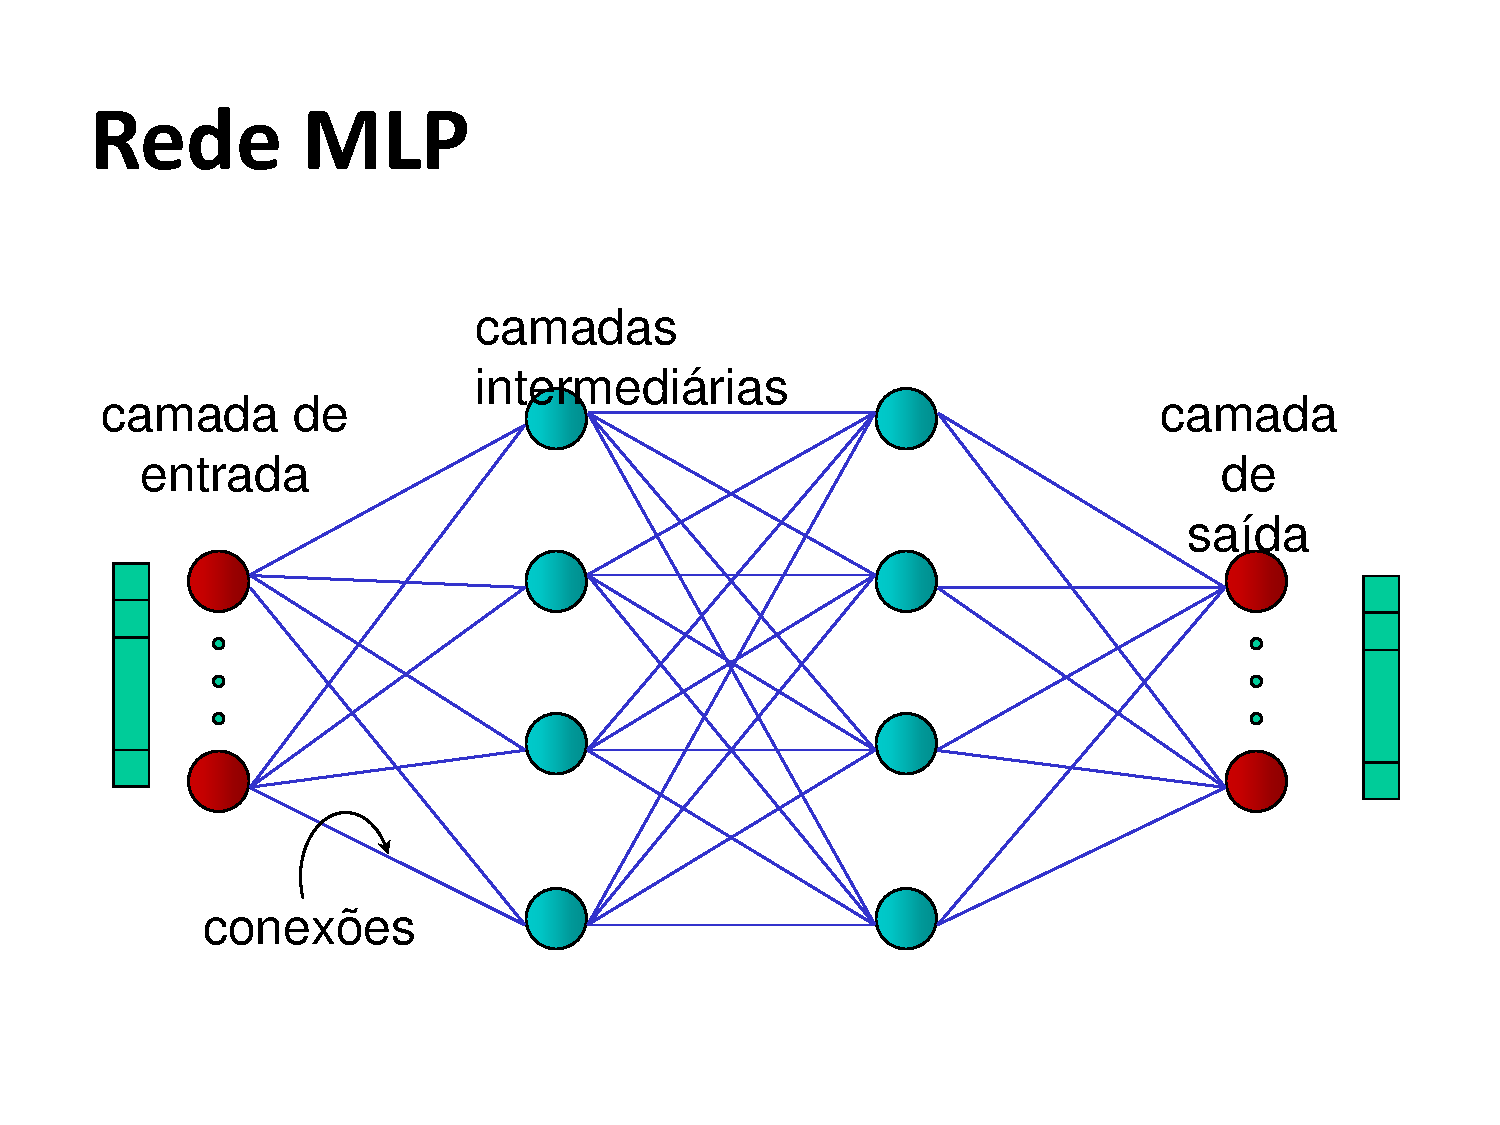
\includepdf[pages=-, frame, scale=0.9]{figs/retropropagacao.pdf}

\begin{frame}{Overfitting em redes neurais}
\begin{columns}[c]
\column{0.5\textwidth}
\begin{itemize}
 \item \textbf{Parada antecipada}: interrompa quando o erro de teste deixa de cair.
 \item \textbf{Regularização L2} nos pesos.
 \item \textbf{\textit{Dropout}}: desliga neurônios aleatoriamente no treino.
 \item \textbf{Aumento de dados}.
\end{itemize}
\column{0.5\textwidth}
\begin{tikzpicture}
\begin{axis}[width=\textwidth, height=0.85\textwidth, axis lines=left, xtick=\empty, ytick=\empty, xlabel={Época}, ylabel={Erro}, ymin=0, ymax=1, xmin=0, xmax=10, legend pos=north east]
\addplot[thick, azul, domain=0:10] {0.9*exp(-0.4*x)+0.02};
\addplot[thick, laranja, domain=0:10] {0.9*exp(-0.5*x)+0.25+0.012*x^2};
\draw[dashed] (axis cs:3.6,0) -- (axis cs:3.6,1);
\node[font=\tiny, rotate=90, anchor=south] at (axis cs:3.6,0.5) {parar aqui};
\legend{Treino, Teste}
\end{axis}
\end{tikzpicture}
\end{columns}
\end{frame}

\begin{frame}[fragile]{Redes na prática}
\begin{lstlisting}
import numpy as np
from sklearn.neural_network import MLPClassifier

X = np.array([[0,0],[0,1],[1,0],[1,1]])
y = np.array([0, 1, 1, 0])          # XOR

mlp = MLPClassifier(hidden_layer_sizes=(4,), activation="tanh",
                    solver="lbfgs", max_iter=2000, random_state=0)
mlp.fit(X, y)
print(mlp.predict(X))               # [0 1 1 0]
\end{lstlisting}
\small Para redes maiores, use PyTorch ou Keras, que treinam em GPU.
\end{frame}

\begin{frame}{Arquiteturas atuais}
\small
\begin{tabularx}{\textwidth}{@{}l X X@{}}
\toprule
\textbf{Arquitetura} & \textbf{Dados típicos} & \textbf{Exemplo de uso} \\
\midrule
Convolucional (CNN) & imagens (ver Aula 3) & diagnóstico por imagem \\
Recorrente e LSTM & sequências & séries temporais \\
\textit{Transformer} & texto, imagem, áudio & modelos de linguagem \\
Difusão & imagens e vídeo & geração de imagens \\
\bottomrule
\end{tabularx}

\vspace{2mm}
\textbf{Limitações}: grande consumo de dados e energia, pouca interpretabilidade e respostas plausíveis porém incorretas.
\end{frame}

\begin{frame}{Exercício}
Use os pesos da rede do XOR e calcule a saída para $\mathbf{x}=(0,0)$.

\pause
\begin{block}{Resposta}
OR: $u=-0{,}5$, logo $h_1=0$. NAND: $u=1{,}5$, logo $h_2=1$. Saída: $u=0+1-1{,}5=-0{,}5$, portanto $y=0$. Correto.
\end{block}
\end{frame}

%%%%%%%%%%%%%%%%%%%%%%%%%%%%%%%%%%%%%%%%
\section{Aprendizado Não Supervisionado}

\begin{frame}{Aprendizado sem rótulos}
\begin{columns}[c]
\column{0.5\textwidth}
Dado apenas $X=\{x_1,\dots,x_n\}\subset\mathbb{R}^d$, buscamos \textbf{estrutura} nos dados.
\begin{itemize}
 \item Agrupamento (\textit{clustering}).
 \item Redução de dimensionalidade.
 \item Detecção de anomalias.
\end{itemize}
\column{0.5\textwidth}
\centering
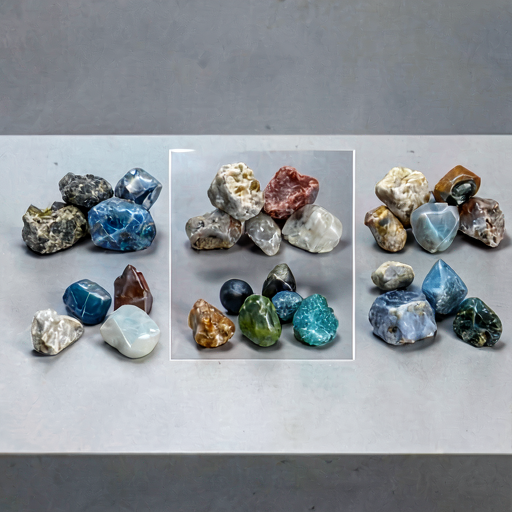
\includegraphics[width=0.8\textwidth]{img/analogia_amostras_agrupadas.png}
{\scriptsize\captionof{figure}{Amostras sem rótulo agrupadas por semelhança.}}
\end{columns}
\begin{reflexao}
\small Como saber se um agrupamento é bom, se não há resposta correta?
\end{reflexao}
\end{frame}

\begin{frame}{K-Means}
Particiona os dados em $k$ grupos que minimizam a soma dos quadrados intragrupo:
\[ \mathcal{J}=\sum_{j=1}^{k}\sum_{x\in C_j}\|x-\mu_j\|^2. \]
\begin{enumerate}
 \item Escolha $k$ centróides iniciais.
 \item Atribua cada ponto ao centróide mais próximo.
 \item Recalcule cada centróide como a média do seu grupo.
 \item Repita até as atribuições não mudarem.
\end{enumerate}
\end{frame}

\begin{frame}{K-Means em três passos}
\centering
\begin{tikzpicture}[scale=0.8]
  \foreach \s/\xo in {0/0, 1/4.2, 2/8.4} {
    \begin{scope}[xshift=\xo cm]
      \draw[gray] (0,0) rectangle (3.6,3);
      \foreach \x/\y in {0.5/0.6,0.8/1.2,0.4/1.9,1.0/0.4,0.9/2.2} \node[ponto, azul] at (\x,\y) {};
      \foreach \x/\y in {2.6/2.4,3.0/1.5,2.8/0.6,2.2/1.0,3.2/2.6} \node[ponto, laranja] at (\x,\y) {};
    \end{scope}
  }
  % passo 1: centróides iniciais
  \node[draw=black, fill=white, star, star points=5, inner sep=1.5pt] at (1.6,2.6) {};
  \node[draw=black, fill=white, star, star points=5, inner sep=1.5pt] at (2.0,0.4) {};
  \node at (1.8,-0.4) {\footnotesize 1. Início};
  % passo 2: atribuição
  \node[draw=black, fill=white, star, star points=5, inner sep=1.5pt] at (5.8,2.6) {};
  \node[draw=black, fill=white, star, star points=5, inner sep=1.5pt] at (6.2,0.4) {};
  \node at (6.0,-0.4) {\footnotesize 2. Atribuir};
  % passo 3: atualização
  \node[draw=black, fill=white, star, star points=5, inner sep=1.5pt] at (9.2,1.3) {};
  \node[draw=black, fill=white, star, star points=5, inner sep=1.5pt] at (11.3,1.6) {};
  \node at (10.2,-0.4) {\footnotesize 3. Atualizar};
\end{tikzpicture}
\end{frame}



\begin{frame}{Limitações e escolha de $k$}
\begin{columns}[c]
\column{0.55\textwidth}
\begin{itemize}
 \item O resultado depende da inicialização, e por isso se usa \textit{k-means++}.
 \item Assume grupos aproximadamente esféricos.
 \item Exige atributos na mesma escala.
 \item \textbf{Escolha de $k$}: método do cotovelo e coeficiente de silhueta
\end{itemize}
\[ s=\frac{b-a}{\max(a,b)} \]
\small $a$: distância média ao próprio grupo. $b$: distância média ao grupo mais próximo.
\column{0.42\textwidth}
\begin{tikzpicture}
\begin{axis}[width=\textwidth, height=0.9\textwidth, axis lines=left, xlabel={$k$}, ylabel={$\mathcal{J}$}, xtick={1,...,7}, ytick=\empty, xmin=1, xmax=7, ymin=0, ymax=10]
\addplot[thick, azul, mark=*, mark size=1.5pt] coordinates {(1,9.5)(2,5.5)(3,2.2)(4,1.8)(5,1.5)(6,1.3)(7,1.2)};
\draw[laranja, dashed] (axis cs:3,0) -- (axis cs:3,2.2);
\end{axis}
\end{tikzpicture}

{\scriptsize Curva ilustrativa. O cotovelo sugere $k=3$.}
\end{columns}
\end{frame}

\begin{frame}{Análise de Componentes Principais (PCA)}
\begin{columns}[c]
\column{0.5\textwidth}
Projeta os dados nas direções de \textbf{maior variância}.
\begin{enumerate}\small
 \item Centralize os dados.
 \item Calcule a matriz de covariância $\Sigma$.
 \item Obtenha autovalores e autovetores, $\Sigma v=\lambda v$.
 \item Projete nos $k$ autovetores de maiores autovalores.
\end{enumerate}
\column{0.5\textwidth}
\begin{tikzpicture}
\begin{axis}[width=\textwidth, height=0.9\textwidth, axis lines=left, xtick=\empty, ytick=\empty, xlabel={$x_1$}, ylabel={$x_2$}, xmin=-3, xmax=3, ymin=-3, ymax=3]
\addplot[only marks, mark=*, mark size=1.4pt, azul] coordinates {(-2.2,-1.8)(-1.6,-1.7)(-1.1,-0.6)(-0.6,-0.9)(-0.2,0.1)(0.3,0.2)(0.7,1.1)(1.2,0.8)(1.7,1.6)(2.1,2.0)(-0.9,-1.1)(0.9,0.5)};
\draw[-{Stealth}, very thick, laranja] (axis cs:-2.4,-2.2) -- (axis cs:2.4,2.2) node[right, font=\scriptsize] {PC1};
\draw[-{Stealth}, thick, verde] (axis cs:0,0) -- (axis cs:-0.8,0.9) node[left, font=\scriptsize] {PC2};
\end{axis}
\end{tikzpicture}
\end{columns}
\end{frame}

\begin{frame}{PCA: exemplo resolvido}
Com $\Sigma=\begin{pmatrix}2&1\\1&2\end{pmatrix}$, os autovalores são $\lambda_1=3$ e $\lambda_2=1$, com autovetores
\[ v_1=\tfrac{1}{\sqrt2}(1,1), \qquad v_2=\tfrac{1}{\sqrt2}(1,-1). \]
A primeira componente explica $\dfrac{3}{3+1}=75\%$ da variância total.

\vspace{2mm}
\small Usos: visualizar dados em duas dimensões, remover redundância e acelerar outros modelos. Para visualização não linear, existem t-SNE e UMAP.
\begin{reflexao}
\small Que informação se perde ao manter apenas PC1?
\end{reflexao}
\end{frame}

\begin{frame}{Exercício}
Aplique o K-Means ($k=2$) aos pontos $1,3,4,10$ com centróides iniciais $\mu_1=1$ e $\mu_2=10$.

\pause
\begin{block}{Resposta}
Atribuição: $C_1=\{1,3,4\}$ e $C_2=\{10\}$. Novos centróides: $\mu_1=8/3\approx2{,}67$ e $\mu_2=10$. A atribuição se repete, então o algoritmo convergiu.
\end{block}
\end{frame}

%%%%%%%%%%%%%%%%%%%%%%%%%%%%%%%%%%%%%%%%
\section{Ética e Síntese}

\begin{frame}{Responsabilidade ao usar ML}
\begin{itemize}
 \item \textbf{Viés nos dados} se transforma em viés nas decisões. Em 2018, a Reuters relatou que a Amazon abandonou uma ferramenta de triagem de currículos que penalizava candidatas.
 \item \textbf{Privacidade}: dados pessoais exigem base legal (LGPD) e proteção.
 \item \textbf{Explicabilidade}: decisões de alto impacto precisam de justificativa.
 \item \textbf{Mudança de contexto}: modelos degradam quando o mundo muda.
\end{itemize}
\begin{reflexao}
\small Quem responde quando um modelo erra em uma decisão sobre pessoas?
\end{reflexao}
\end{frame}

\begin{frame}{Resumo da aula}
\small
\begin{tabularx}{\textwidth}{@{}l X X@{}}
\toprule
\textbf{Tema} & \textbf{Ideia central} & \textbf{Pergunta-chave} \\
\midrule
Supervisionado & aprender $x\mapsto y$ com exemplos & o modelo generaliza? \\
Teste & separar treino e teste & há vazamento de dados? \\
Classificação & matriz de confusão e métricas & qual erro custa mais? \\
Regressão & mínimos quadrados e resíduos & as suposições valem? \\
Redes neurais & camadas, perda e gradiente & o que aprendeu, e com que custo? \\
Não supervisionado & agrupar e reduzir dimensões & a estrutura faz sentido? \\
\bottomrule
\end{tabularx}
\end{frame}

%%%%%%%%%%%%%%%%%%%%%%%%%%%%%%%%%%%%%%%%
\section{Referências}

\begin{frame}[t,allowframebreaks]{Referências}
\footnotesize
\begin{thebibliography}{99}
\bibitem{A01} Russell, S. e Norvig, P. (2021). \textit{Artificial Intelligence: A Modern Approach}. 4ª ed. Pearson.
\bibitem{A02} Géron, A. (2022). \textit{Hands-On Machine Learning with Scikit-Learn, Keras, and TensorFlow}. 3ª ed. O'Reilly.
\bibitem{A03} Goodfellow, I., Bengio, Y. e Courville, A. (2016). \textit{Deep Learning}. MIT Press.
\bibitem{A04} Chollet, F. (2021). \textit{Deep Learning with Python}. 2ª ed. Manning.
\bibitem{A05} James, G. et al. (2021). \textit{An Introduction to Statistical Learning}. 2ª ed. Springer.
\bibitem{A06} Mitchell, T. (1997). \textit{Machine Learning}. McGraw-Hill.
\bibitem{A07} McCulloch, W. e Pitts, W. (1943). A logical calculus of the ideas immanent in nervous activity. \textit{Bulletin of Mathematical Biophysics}, 5.
\bibitem{A08} Rosenblatt, F. (1958). The perceptron. \textit{Psychological Review}, 65(6).
\bibitem{A09} Rumelhart, D., Hinton, G. e Williams, R. (1986). Learning representations by back-propagating errors. \textit{Nature}, 323.
\bibitem{A10} Vaswani, A. et al. (2017). Attention is all you need. \textit{NeurIPS}.
\end{thebibliography}
\end{frame}

\setbeamertemplate{logo}{}
\begin{frame}
\titlepage
\end{frame}

\end{document}
